%!TEX root = ../report.tex

\section{Firewalls and Security Policies}
We define a system as secure if, started in an allowed state, always stays in states that are allowed.

\subsection{The three Security Components}
\begin{itemize}
  \item \textbf{Requirements} define security goals
  \item \textbf{Policy} are rules to implement the requirements
  \item \textbf{Mechanisms} enforce the policy
\end{itemize}

\subsection{Network Firewalls}
Firewalls provide \textbf{controlled access} at the network level to resources.
They are usually deployed where a protected subnet is connected to a less trusted network like the internet (c.f.\ Figure~\ref{fig:firewall_placement}).
From the firewall's point of view, there are incoming and outgoing packet on all interfaces.
These can be filtered using two different strategies.\\
\textbf{Whitelisting}, which is considered as the best practice, has the default behavior of denying all packets and allowing only explicitly permitted ones whereas \textbf{blacklisting} allows everything except blocked packets.


\begin{figure}[h]
  \centering
  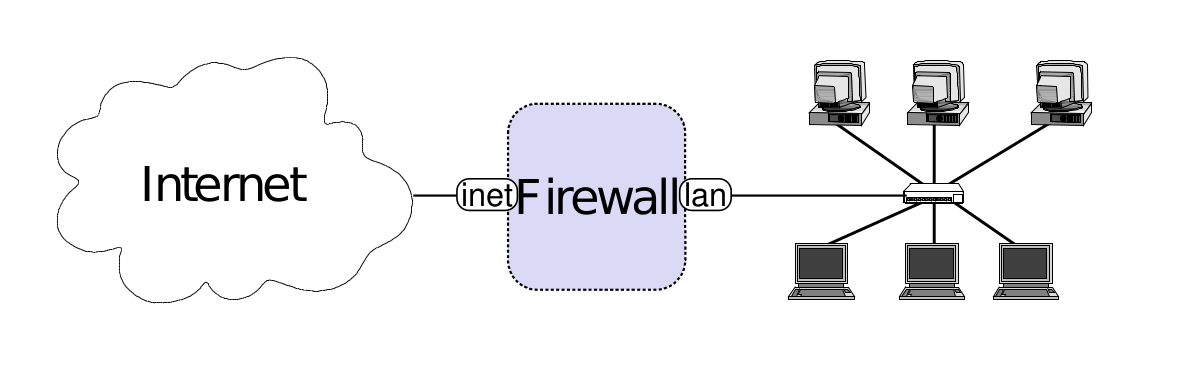
\includegraphics[width=.8\textwidth]{figures/firewall_placement.png}
  \caption{Firewall Placement}\label{fig:firewall_placement}
\end{figure}

\subsubsection*{Configuring Firewalls}
Firewalls are configured with rulesets which are traversed sequentially until a matching one is found.
Those rules are composed of a matching condition and an action.
Possible actions are for example accept, drop, reject or log.
The matching conditions are a bit more complex.
They include the incoming interface, several layer 2 to 4 packet fields (srcMAC, dstMAC, srcIP, dstIP, prot, srcPort, dstPort, flags,\dots), states (in case of stateful matching) and other relevant conditions.

\subsubsection*{Stateful Firewalls}
Stateful Firewalls keep states of connections with the help of IP-5-Tuples (srcIP, dstIP, protocol, srcPort, dstPort).
A new state is generated when a packet with a new tuple arrives which transitions from NEW to ESTABLISHED state.
It is usually advisable to put more frequently used rules to the top of the firewall, i.e.\ matching established connections (new connections are rarer) and to check that ports are above the well defined port range ($\geq 1024$).
Figure~\ref{fig:stateful_firewall} shows an example of a stateful firewall configuration.
\begin{figure}[h]
  \centering
  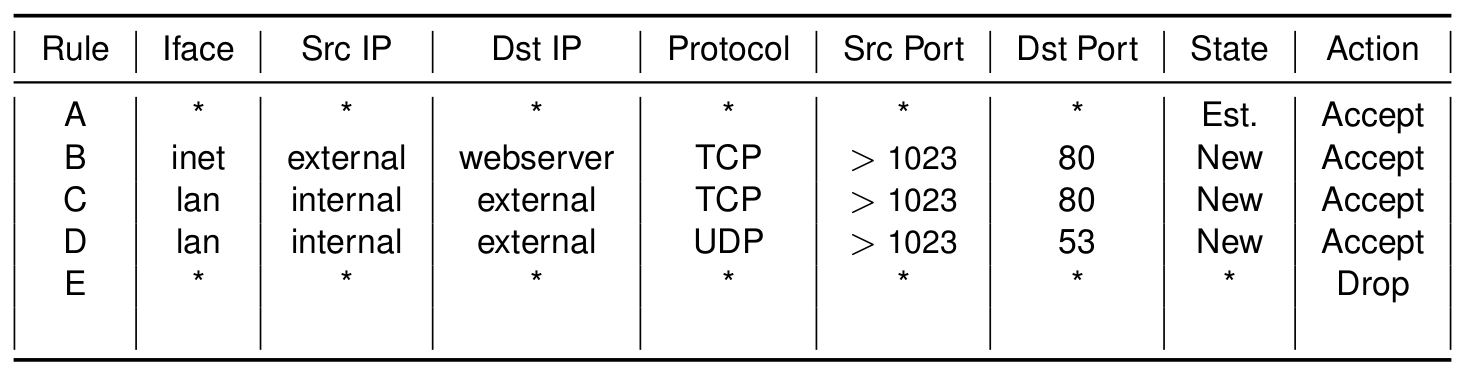
\includegraphics[width=.8\textwidth]{figures/stateful_firewall.png}
  \caption{Stateful Firewall Configuration}\label{fig:stateful_firewall}
\end{figure}

\subsubsection*{Stateless Firewalls}
Stateless firewalls do not generate states for incoming connections but only operate on single packets since keeping states is expensive and needs fast memory.
For this reason lookup times are in $\mathcal{O}(\#rules)$ which, for large $\#rules$ is slower than stateful filtering ($\mathcal{O}(1)$).
For small $\#rules$ stateless filtering is faster though due to the lack of memory writes.
It is also more complex to configure which makes the approach more error prone.
An example for a stateless ruleset is shown in Figure~\ref{fig:stateless_firewall}.
\begin{figure}[h]
  \centering
  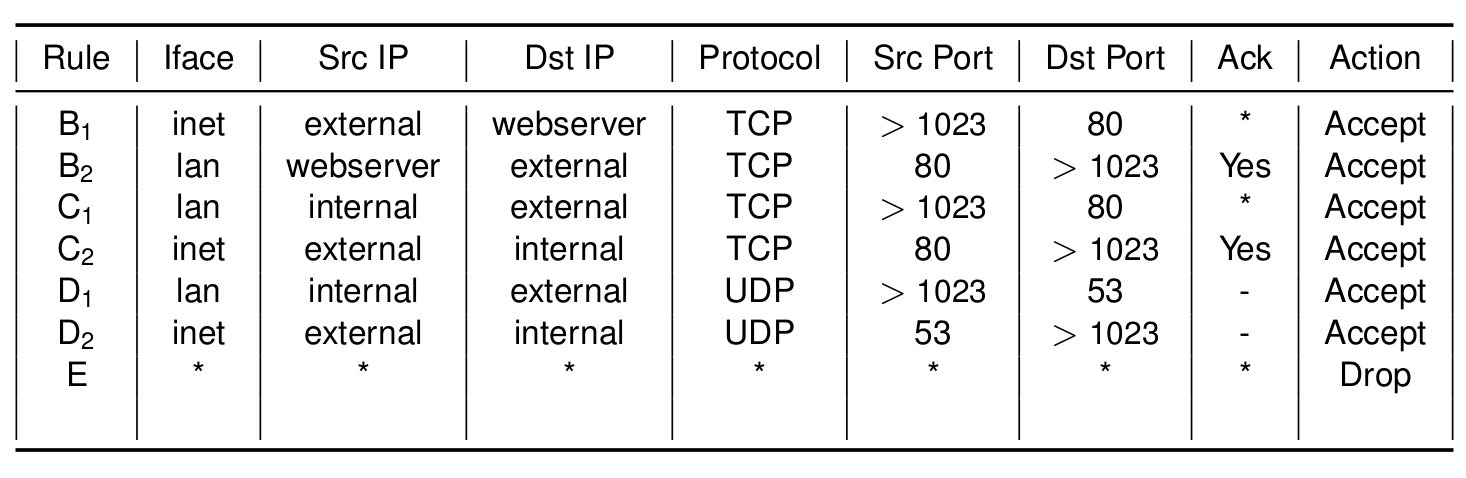
\includegraphics[width=.8\textwidth]{figures/stateless_firewall.png}
  \caption{Stateless Firewall Configuration}\label{fig:stateless_firewall}
\end{figure}

Stateless firewalls usually look at the ACK flag of TCP connection to determine approximately if connections are new or established.
When a SYN/ACK packet is sent as first packet of a connection, the firewall will pass it but the host will drop it if implement properly.

\subsubsection*{Spoofing Protection}
Spoofing is the forgery of IP addresses by filling the source IP field with another IP than one's own.
Spoofing protection then allows only IP addresses that belong to you on outgoing connections.
For incoming traffic this is more difficult since we can not determine where the packet actually came from so we are only able to block our and special purpose IPs.

\subsubsection*{Common Errors}
\begin{itemize}[noitemsep, topsep=0pt]
  \item How is your firewall management interface reachable?
  \item What is allowed over the Internet?
  \item IPv4 and IPv6?
  \item Outbound rule ANY? (c.f.\ spoofing)
  \item Policy’s vs. Firewalls understanding of Inbound and Outbound?
  \item Shadowing: unreachable firewall rules
\end{itemize}

\subsubsection*{What Firewalls cannot do}
\begin{itemize}[noitemsep, topsep=0pt]
  \item can’t protect against malicious insiders
  \item can’t protect against connections that don’t go through it
  \item can’t protect against completely new threats
  \item can’t fully protect against viruses
  \item does not perform cryptographic operations, e.g.\ message authentication
  \item can’t set itself up correctly
\end{itemize}

\subsubsection*{Bastion Hosts}
A bastion host is a host that is more exposed to the hosts of an external network than the other hosts of the network it protects.
When configuring, one should keep in mind that it might get compromised so do things like disabling SSH password login, do not allow it to sniff internal traffic or disable user accounts.

\subsubsection*{Firewall Architectures}
\begin{description}
  \item[Simple Packet Filter Architecture] Packet filtering is done through a filtering router or firewall with two interfaces.
    \begin{figure}[H]
      \centering
      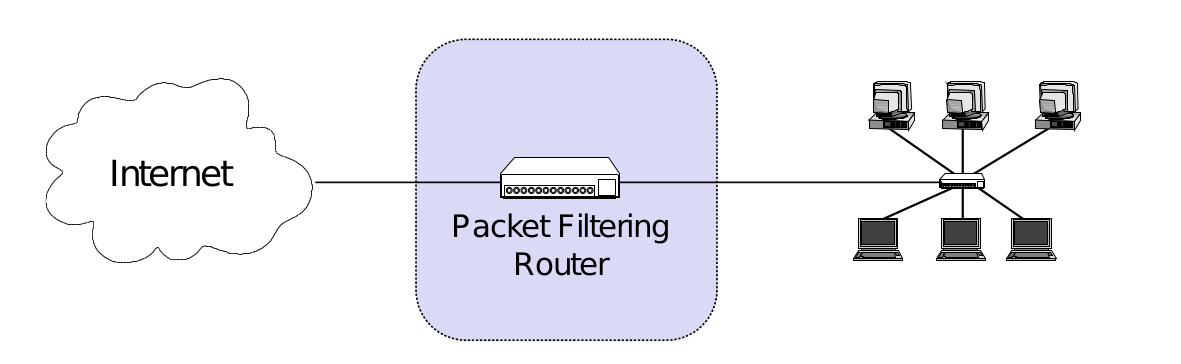
\includegraphics[width=.8\textwidth]{figures/firewall_simple_packet_filter_architecture.png}
    \end{figure}
  \item[Dual-Homed Host Architecture] The bastion host is part of two networks and is firewall and application proxy.
    Disadvantage: bastion host is bottleneck
    \begin{figure}[H]
      \centering
    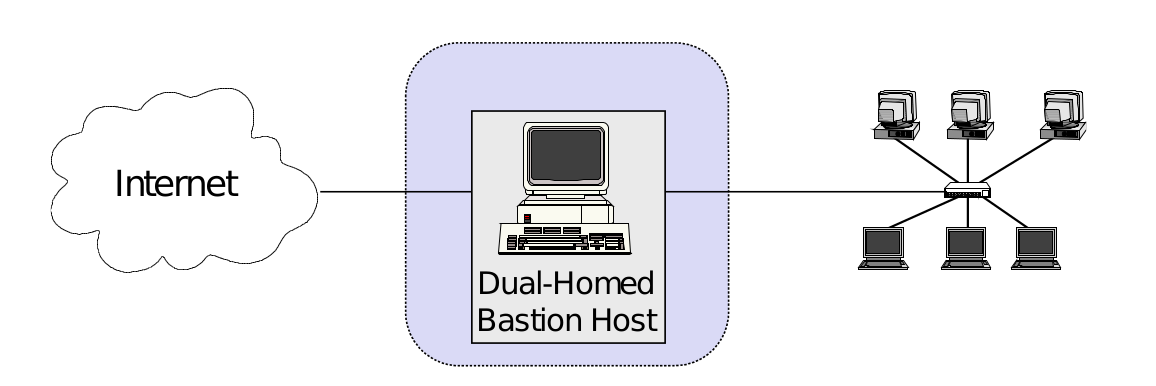
\includegraphics[width=.8\textwidth]{figures/firewall_dual-homed_host_architecture}
    \end{figure}
  \item[Screened Host Architecture] The bastion host is proxy, located in the internal network and thus protected by the firewall.
    \begin{figure}[H]
      \centering
      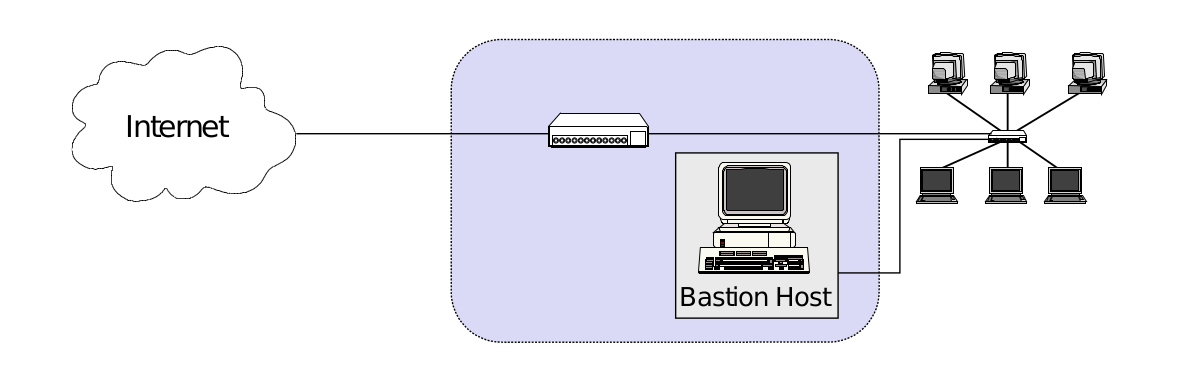
\includegraphics[width=.8\textwidth]{figures/firewall_screening_host_architecture.png}
    \end{figure}
  \item[Screened Subnet Architecture - DMZ] A demilitarized zone (DMZ) is configured hosting the bastion host (proxy) and publicly accessible servers.
    The second packet filter is an additional protection measurement in case the DMZ gets compromised.
    \begin{figure}[H]
      \centering
      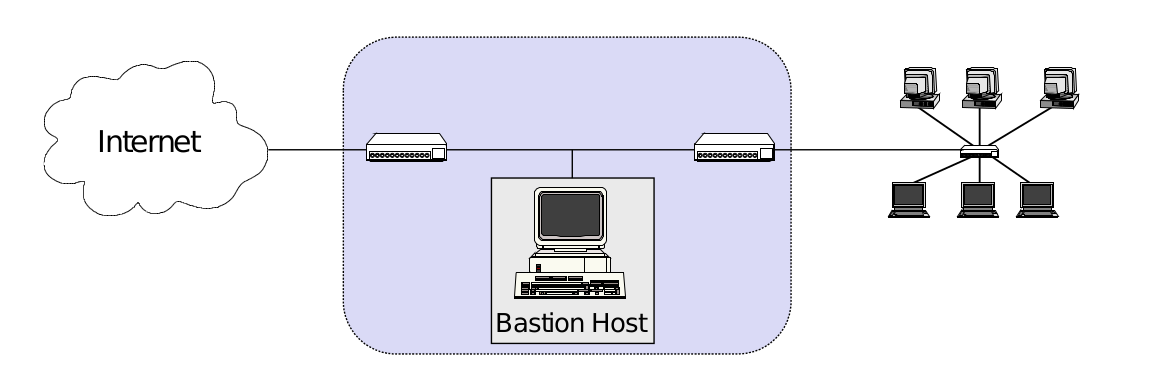
\includegraphics[width=.8\textwidth]{figures/firewall_screened_subnet_architecture.png}
    \end{figure}
\end{description}
